In order to prepare the SVT for real physics data-taking we calibrated the readout system.
This involves extraction of the mean baseline (pedestal), baseline noise and gain for each of the 
12,780 SVT channels. All measurements are made with the APV25 chips configured to the nominal 
operating points {\color{red} reference from pac39} and all sensors biased to 180~V. 
The APV25 chips are being operated in multi-peak mode with six samples being readout per trigger 
allowing us to extract the  t$_{0}$ and amplitude of the signal being read out.


Figure~\ref{fig:baseline_and_gain} shows an intensity plot of the pedestals across a sensor where the noise is represented 
by the width if the band and falling into the expected range of about 35~ADC counts or 950~$e^{-}$ 
{\color{red} check this}. The baseline variations are subtracted out and the noise was observed to 
be consistently within $31-35$~ADC counts or $X-Ye^{-}$ across single chips and 
different modules in the detector. One feature observed are large noise values for the channels 
at the edge of the chip. This was also reported by the CMS collaboration and is still under 
investigation.
\begin{figure}[]
	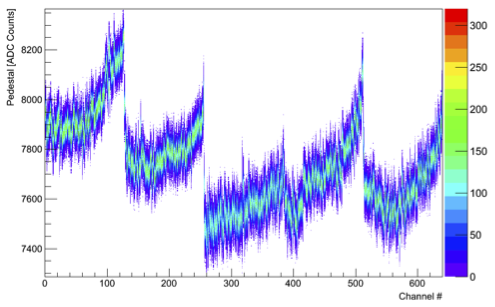
\includegraphics[width=0.45\textwidth]{test2012/svtperformance/baseline}
	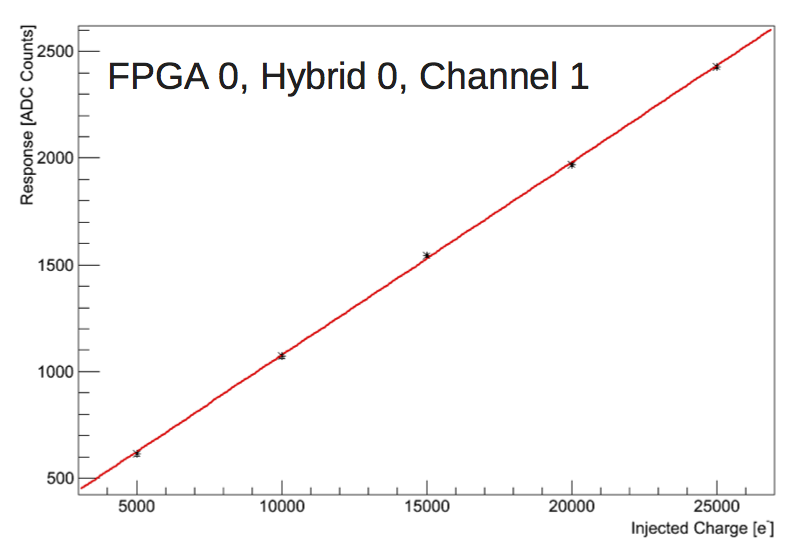
\includegraphics[width=0.45\textwidth]{test2012/svtperformance/gain}
	\caption{\small{The baseline across a hybrid (left) and the measured response as a function of 
	input charge (right). The overall shifts in the baseline are calibrated out where distinct edges 
	are associated with the five APV25 chips on the hybrid. The gain shows good linearity up to 
	about three $mip$s.} {\color{red}Should we show noise instead of baseline?}}
	\label{fig:baseline_and_gain}
\end{figure}
Another important aspect for the characterization of the SVT is the response and the associated 
gain. Using the APV25 internal calibration circuit a known fixed charge was injected into all 
channels of the which allows for an accurate determination of the response and its 
scaling with input charge, shown in Fig.~\ref{fig:baseline_and_gain}. The gain uniformity was 
within the expected range across chips and modules and show good linearity of charge 
depositions up to about 3 $mip$s. 

The hits on each single sensor in the SVT are processed to form clusters of energy depositions. 
The average pulse shape in our test run data for each cluster associated to a track and the 
measured amplitude are shown in Fig.~\ref{foig:pulseshape} demonstrating 
the expected Landau distribution. 
\begin{figure}[]
	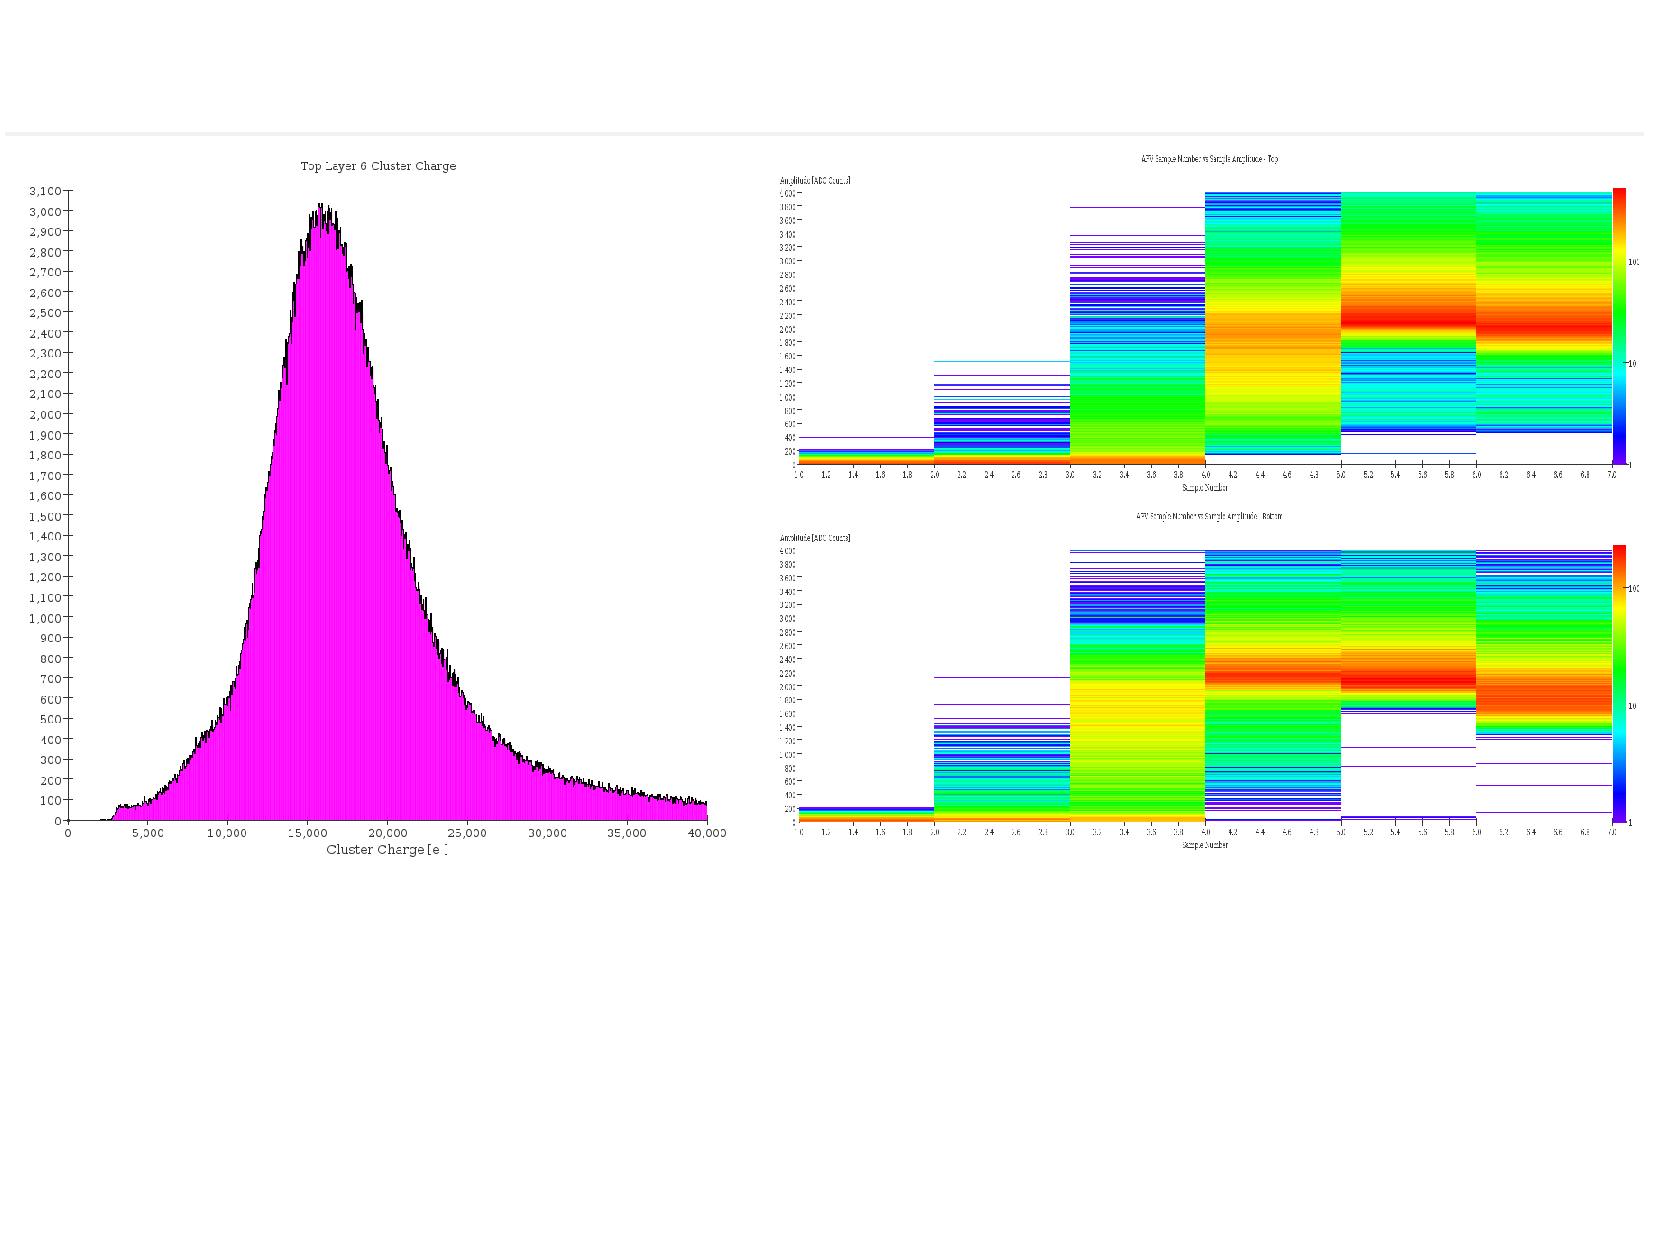
\includegraphics[width=\textwidth]{test2012/svtperformance/pulseshape_and_landau}
	\caption{\small{The distribution of cluster amplitudes (left) showing the characteristic Landau 
	shape and the pulse shape from the six samples readout (right) {\color{red} Remove one of the pulse shapes}. }}
	\label{fig:pulseshape}
\end{figure}

The noise and response measured with the detector show a good signal to noise ratio of 25 
{\color{red} check this.} well matched to the expected behavior. Besides shown the $mip$ 
signal the six sample readout shows that the trigger system described below is well timed in 
with the tracker. 

As described in Sec.~\ref{sec:svt} the six sample readout is crucial in order to time-correlate 
hits in the tracker to lower the confusion rate in the pattern recognition during electron running. 
The time reconstruction algorithm described in \ref{sec:svt} was used to fit a single hit to each SVT channel in each event. The fit quality $\chi^2$ was shown to agree with the expected distribution 
for four degrees of freedom for an ideal $CR-RC$ function. 
%\begin{figure}[]
%	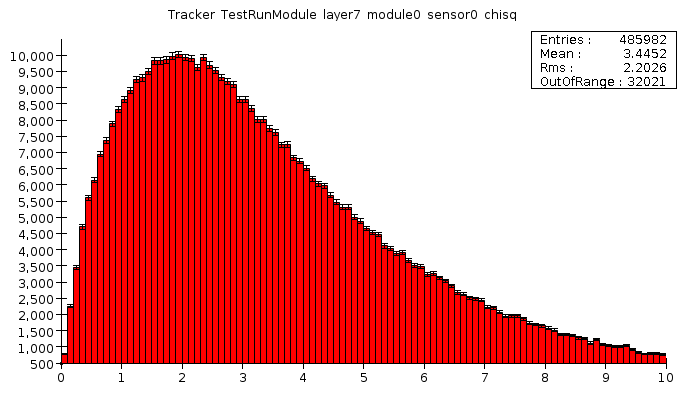
\includegraphics[width=0.6\textwidth]{test2012/svtperformance/apvfit_chisq}
%	\caption{\small{Histogram of $\chi^2$ values for pulse fits for all channels on a representative sensor. The peak at 2 is consistent with 4 degrees of freedom (2 fit parameters), as expected. Pileup was not considered due to the very low hit rate in 
%the SVT in this photon beam test. } }
%	\label{fig:apvfit}
%\end{figure}
After clustering hits on a sensor, the hit time for the each cluster is computed as the 
amplitude-weighted average of the channel hit times. Since we have no measurement of the ``true'' hit time, we study the overall SVT hit 
timing performance using the average of all cluster times in a track as the ``track time,'' and take the
 residual of the cluster time relative to that. The observed track time , shown in Figure \ref{fig:tracktime}, has the expected amount of trigger jitter due to the readout clock and trigger 
 system jitter. After correcting for offsets for each sensor (time-of-flight, clock phase) the RMS 
 of the final residual distribution is roughly 2.4~ns for each sensor. 
\begin{figure}[ht]
	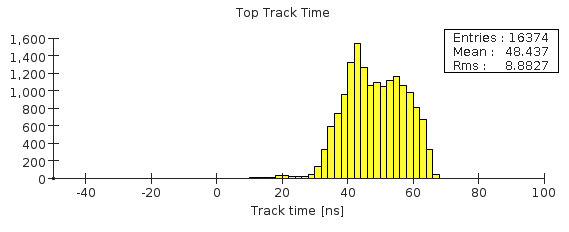
\includegraphics[width=0.7\textwidth]{test2012/svtperformance/track_time_top}
	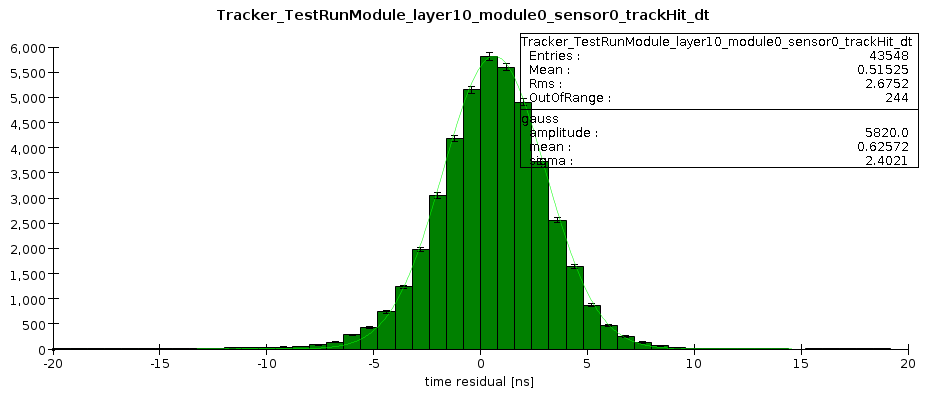
\includegraphics[width=0.7\textwidth]{test2012/svtperformance/timeres}
	\caption{\small{Track time distribution (top) and cluster time residual (bottom). The 
	track time is measured relative to the APV25 clock. The width of the distribution is due to 
	trigger jitter (24 ns jitter in tracker readout clock, plus 16 ns jitter in the trigger system). 
	The cluster time residual is for a representative sensor relative to the track time.}}
	\label{fig:tracktime}
\end{figure}
Because the track time is calculated using the individual hit times, the hit time is positively correlated 
with the track time; thus the RMS of the residual is slightly smaller than the true time resolution.
The standard deviation of this residual for $n$-hit tracks where all hits have the same time resolution 
is reduced by a factor of $\sqrt{(n-1)/n}$; since most of our tracks have 8 clusters, the true time 
resolution is 2.6 ns. 
%\begin{figure}[ht]
%	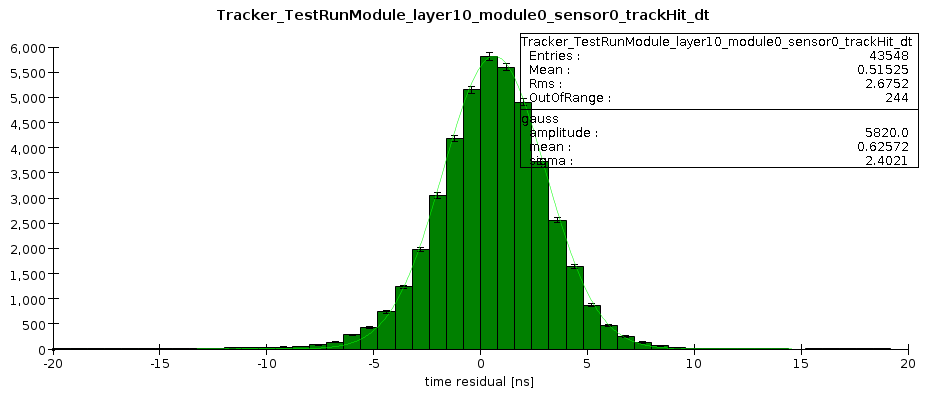
\includegraphics[width=\textwidth]{test2012/svtperformance/timeres}
%	\caption{\small{Histogram and Gaussian fit of residual of cluster times for a representative sensor, relative to the track time. Because the cluster times and track time have positive covariance, the true time resolution is slightly larger than the standard deviation shown here.} }
%	\label{fig:timeres}
%\end{figure}
%\begin{figure}[ht]
%	\includegraphics[width=\textwidth]{test2012/svtperformance/hit_dt}
%	\caption{\small{} }
%	\label{fig:hit_dt}
%\end{figure}

This is somewhat worse than the $\approx 2$ ns resolution expected (see Fig.~\ref{fig:timeres} in 
Sec.~\ref{sec:performance}, but we believe this discrepancy is due to our fit function. Our pulse 
shape fit assumes an ideal CR-RC pulse shape; since the actual pulse shape has a slower rise time, 
there is a systematic pull on the hit time when a hit comes immediately before the APV clock time. 
This is visible in Figure \ref{fig:timeres_2D} as a shift in the residual at certain values of track time.
\begin{figure}[]
	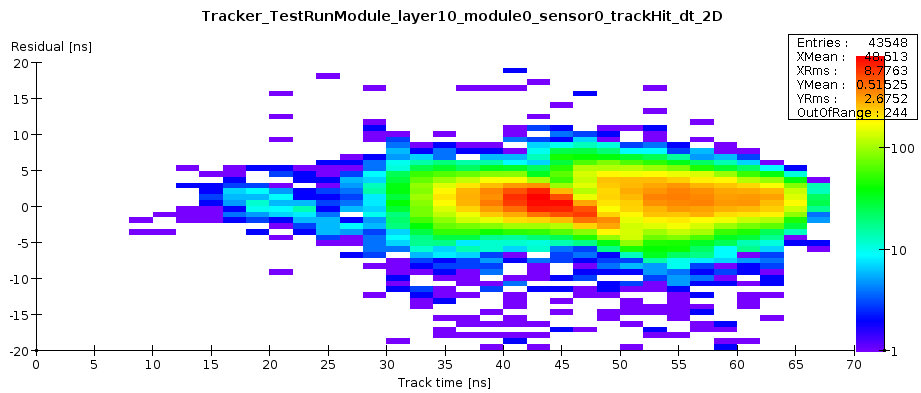
\includegraphics[width=0.7\textwidth]{test2012/svtperformance/timeres_2D}
	\caption{\small{Plot of the time residual for a representative sensor vs. the track time. 
		The kinks in the horizontal band are caused by the fitter; without them the 1-D histogram in Figure \ref{fig:timeres} (the projection of this histogram) would be narrower.} }
	\label{fig:timeres_2D}
\end{figure}
Work is in progress to use the actual pulse shape in time reconstruction; this should improve time resolution to that expected from previous studies. 
It should be noted that the demonstrated time resolution above is still adequate to achieve a good 
enough rejection due to pile-up hits in the HPS electron run. 




\vspace{1cm}{\bf Tracking algorithms [Matt/Omar]}


Pattern recognition/Stereo hit reconstruction and description of the tracking algorithm. 

Plots: tracking efficiency vs run nr, hit efficiency vs run nr for data. Overlay MC.

\vspace{1cm}{\bf Two track events analysis [Matt]}

Analysis of two track events. 

Plots: invariant mass, vertex position, 2-track event multiplicity. Compare with MC for all these 


\vspace{1cm}{\bf SVT DAQ Performance [Pelle/Omar/Ryan]}
General discussion on SVT rates, event size.

Plots: 
